\newpage
\section{Билет 17. Безразмерные параметры, определяющие характер движения несжимаемой вязкой жидкости. Число Рейнольдса. Предельные случаи. Пограничный слой.}

Источник: \url{https://pstu.ru/files/2/file/kafedra/fpmm/of/Kolesnichenko_V.I._Vvedenie_v_mehaniku_nesjimaemoyi_jidkosti.pdf}

\subsection{Безразмерные параметры}
Будем рассматривать для примера двумерное (плоское) движение и теплоперенос вязкой несжимаемой жидкости. Оно характеризуется системой уравнений:
\begin{equation}
    \begin{cases}
        \frac{\partial v_x}{\partial t} + v_x\frac{\partial v_x}{\partial x} + v_y\frac{\partial v_x}{\partial y} = -\frac{1}{\rho} \frac{\partial p}{\partial x} + \nu (\frac{\partial^2 v_x}{\partial x^2} + \frac{\partial^2 v_x}{\partial y^2})\\

        \frac{\partial v_y}{\partial t} + v_x\frac{\partial v_y}{\partial x} + v_y\frac{\partial v_y}{\partial y} = -\frac{1}{\rho} \frac{\partial p}{\partial y} + \nu (\frac{\partial^2 v_y}{\partial x^2} + \frac{\partial^2 v_y}{\partial y^2})\\

        \frac{\partial v_x}{\partial x} + \frac{\partial v_y}{\partial y} = 0\\

        \frac{\partial T}{\partial t} + v_x\frac{\partial T}{\partial x} + v_y\frac{\partial T}{\partial y} = \alpha(\frac{\partial^2 v_x}{\partial x^2} + \frac{\partial^2 v_x}{\partial y^2})\\
    \end{cases}
\end{equation}

Здесь:
\begin{enumerate}
    \item[\textbullet] $v$ - скорость потока
    \item[\textbullet] $p$ - давление
    \item[\textbullet] $\nu$ - кинематическая вязкость 
    \item[\textbullet] $\alpha$ - коэффициент температуропроводности
    \item[\textbullet] $T$ - температура
\end{enumerate}

\bigskip
Введем следующие характерные величины:
\begin{enumerate}
    \item[\textbullet] $L$ - геометрический размер, например, диаметр цилиндрического канала
    \item[\textbullet] $v_0$ - скорость, например, скорость на оси канала или набегающего потока
    \item[\textbullet] $p_0$ - давление, например, на входе в канал
    \item[\textbullet] $t_0 = \frac{L}{v_0}$ - временной масштаб задачи
    \item[\textbullet] $T_h - T_c$ -  разность температур, например, горячей и холодной стенок полости
\end{enumerate}

С помощью введенных характерных величин определим безразмерные переменные (будем обозначать их буквами с верхним значком «тильда»), которые свяжем со старыми размерными переменными:

$$\Tilde{x} = \frac{x}{L},\; \Tilde{y} = \frac{y}{L},\; \Tilde{v_x} = \frac{v_x}{v_0},\; \Tilde{v_y} = \frac{v_y}{v_0},\; \Tilde{p} = \frac{p}{p_0},\; \Tilde{t} = t_0\frac{v_0}{L},\; \Tilde{\theta} = \frac{T - T_h}{T_h - T_c}$$

$$\frac{\partial}{\partial \Tilde{t}} = \frac{l}{v_0} \frac{\partial}{\partial t},\; \frac{\partial}{\partial \Tilde{x}} = l \frac{\partial}{\partial x},\; \frac{\partial^2}{\partial \Tilde{x}^2} = l^2 \frac{\partial}{\partial x^2}\;\; (and\; so\; on...)$$

Тогда обезразмеренное уравнение [1] нашей исходной системы переписывается в виде:

$$\frac{v_0L}{\nu} (\frac{\partial \Tilde{v_x}}{\partial \Tilde{t}} + \Tilde{v_x}\frac{\partial \Tilde{v_x}}{\partial \Tilde{x}} + \Tilde{v_y}\frac{\partial \Tilde{v_x}}{\partial \Tilde{y}}) = -\frac{p_0L}{\rho \nu v_0} \frac{\partial \Tilde{p}}{\partial \Tilde{x}} + (\frac{\partial^2 \Tilde{v_x}}{\partial \Tilde{x}^2} + \frac{\partial^2 \Tilde{v_x}}{\partial \Tilde{y}^2})$$

Коэффициент в левой части называется \textbf{числом Рейнольдса}:
$$Re = \frac{v_0L}{\nu}$$

Число Рейнольдса есть мера отношения сил инерции, действующих в потоке, к силам вязкости. При малых значениях $Re$ преобладают силы вязкости, при больших – силы инерции.

\bigskip
Преобразуем коэффициент в правой части:
$$\frac{p_0L}{\rho \nu v_0} = \frac{v_0L}{\nu} \cdot \frac{p_0}{\rho v_0^2} = Re \cdot Eu,$$
где коэффициент $$Eu = \frac{p_0}{\rho v_0^2}$$
называется \textbf{числом Эйлера}. Он описывает отношение между силами давления на единичный объём жидкости и инерционными силами.

\bigskip
Выразим $T = T_h + \theta (T_h - T_c)$ и обезразмерим уравнение [4] нашей исходной системы:

$$\frac{v_0L}{\alpha} (\frac{\partial \Tilde{\theta}}{\partial \Tilde{t}} + \Tilde{v_x}\frac{\partial \Tilde{\theta}}{\partial \Tilde{x}} + \Tilde{v_y}\frac{\partial \Tilde{\theta}}{\partial \Tilde{y}}) = (\frac{\partial^2 \Tilde{\theta}}{\partial \Tilde{x}^2} + \frac{\partial^2 \Tilde{\theta}}{\partial \Tilde{y}^2})$$

Коэффициент в левой части называется \textbf{числом Пекле}. Оно равно отношению конвективного теплопереноса к теплопроводному:
$$Re = \frac{v_0L}{\alpha}$$

Его также можно переписать в виде:
$$Re = \frac{v_0L}{\nu} \cdot \frac{\nu}{\alpha} = Re \cdot Pr,$$

где $Pr = \frac{\nu}{\alpha}$ называется \textbf{числом Прандтля}


\subsection{Пограничный слой}

Рассмотрим гидродинамические и тепловые процессы в пристенном слое жидкости. Скорость тончайшего слоя жидкости, непосредственно прилегающего к поверхности твердого тела, равна нулю, т.е. выполняется так называемое \textbf{условие прилипания}. 

Рассмотрим продольное обтекание плоской твердой поверхности тела безграничным потоком жидкости (см. рисунок). Пусть скорость набегающего потока постоянна и равна $v_0$ . Около пластины образуется слой заторможенной жидкости, в пределах которого скорость изменяется от нуля на поверхности до $v_0$ вдали от тела. Этот слой называется гидродинамическим \textbf{пограничным слоем}.

\begin{figure}[h]
    \centering
    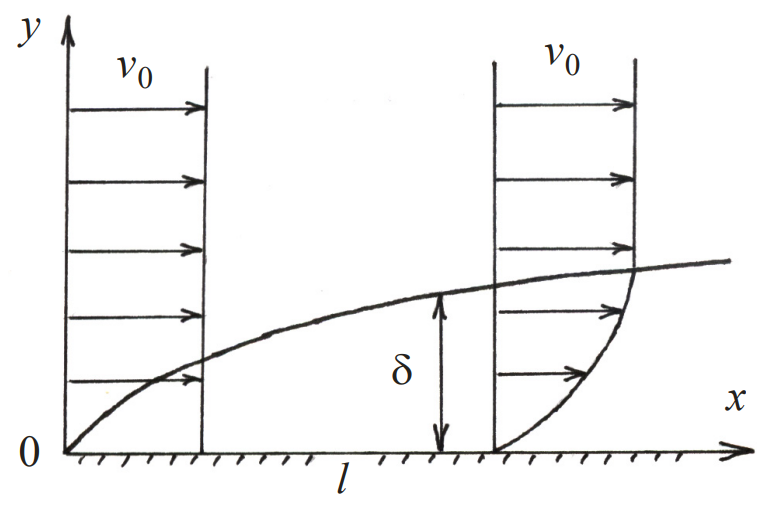
\includegraphics[scale=0.5]{17/fig_17_1.png}
    \caption{Пограничный слой}
\end{figure}

Толщина пограничного слоя $\delta$ – понятие довольно условное, так как резкого перехода от погранслоя к течению вне слоя
нет. Поэтому принимают под $\delta$ такое расстояние от стенки, при котором $v_x$ отличается от $v_0$ на заданную малую величину $\epsilon << 1$, например, $v_x = (1-\epsilon)v_0$ при $y=\delta$. Если $l$ – характерная длина пластины вдоль оси $OX$, то справедливо неравенство $\delta << l$.

\bigskip
При омывании пластины поток жидкости как бы разделяется на две части: пограничный слой, для которого справедливо условие
$$\frac{\partial v_x}{\partial y}\Big|_{y<\delta} \neq 0$$

и внешний поток, в котором $\frac{\partial v_x}{\partial y} = 0$; $v_x = v_0$ при $y \geq \delta$.

\bigskip
Во внешнем потоке, где число Рейнольдса $Re >> 1$, преобладают силы инерции, вязкостные силы здесь не проявляются, т.е. жидкость можно считать идеальной. Напротив, в пограничном слое силы вязкости и инерционные силы соизмеримы.

Явления, происходящие в пограничном слое, служат источником гидродинамического сопротивления при движении тел в жидкостях.

\bigskip
Распишем уравнения движения для двумерного стационарного потока жидкости:

\begin{equation}
    \begin{cases}
        v_x\frac{\partial v_x}{\partial x} + v_y\frac{\partial v_x}{\partial y} = -\frac{1}{\rho} \frac{\partial p}{\partial x} + \nu (\frac{\partial^2 v_x}{\partial x^2} + \frac{\partial^2 v_x}{\partial y^2})\\

        v_x\frac{\partial v_y}{\partial x} + v_y\frac{\partial v_y}{\partial y} = -\frac{1}{\rho} \frac{\partial p}{\partial y} + \nu (\frac{\partial^2 v_y}{\partial x^2} + \frac{\partial^2 v_y}{\partial y^2})\\

        \frac{\partial v_x}{\partial x} + \frac{\partial v_y}{\partial y} = 0\\
    \end{cases}
\end{equation}

Ввиду малости толщины пограничного слоя $\delta$ принимаем, что поперек него давление не изменяется ($\frac{\partial p}{\partial y} = 0$). Также будем рассматривать так называемое \textbf{безградиентное течение}, в котором в области пограничного слоя $\frac{\partial p}{\partial x} = 0$.

Проведём оценку порядков величин и слагаемых, входящих в рассматриваемую систему:
$$x = O(l),\; y = O(\delta),\; v_x = O(v_0)$$
$$\frac{\partial}{\partial x} = O(\frac{1}{l}),\; \frac{\partial^2}{\partial x^2} = O(\frac{1}{l^2}),\; \frac{\partial}{\partial y} = O(\frac{1}{\delta}),\; \frac{\partial^2}{\partial y^2} = O(\frac{1}{\delta^2})$$

Оценим величину $v_y$. Из уравнения неразрывности имеем $O(\frac{\partial v_x}{\partial x}) = O(\frac{\partial v_y}{\partial y})$ или $\frac{v_0}{l} = \frac{O(v_y)}{\delta}$, откуда получаем:
$$O(v_y) = v_0\frac{\delta}{l}$$

Оценим теперь порядки отдельных слагаемых первого уравнения системы:
$$v_x\frac{\partial v_x}{\partial x} = O(\frac{v_0^2}{l}),\; v_y\frac{\partial v_x}{\partial y} = O(v_0\frac{\delta}{l} \frac{v_0}{\delta}) = O(\frac{v_0^2}{l})$$
$$\nu \frac{\partial^2 v_x}{\partial x^2} = O(\nu \frac{v_0}{l^2}),\; \nu \frac{\partial^2 v_x}{\partial y^2} = O(\nu \frac{v_0}{\delta^2})$$

Видим, что отношение вязкостных членов равно $O(\nu \frac{v_0}{l^2}) : O(\nu \frac{v_0}{\delta^2}) = O(\frac{\delta^2}{l^2})$.

Поскольку для пограничного слоя $\delta << l$, то вязкостным членом можно пренебречь.

\bigskip
Оценим аналогично порядки отдельных слагаемых второго уравнения системы: 
$$v_x\frac{\partial v_y}{\partial x} = O(\frac{v_0^2}{l}\frac{\delta}{l}),\; v_y\frac{\partial v_y}{\partial y} = O(\frac{v_0^2}{l}\frac{\delta}{l})$$
$$\nu \frac{\partial^2 v_y}{\partial x^2} = O(\nu \frac{v_0}{l^2}\frac{\delta}{l}),\; \nu \frac{\partial^2 v_y}{\partial y^2} = O(\nu \frac{v_0}{\delta^2}\frac{\delta}{l})$$

Все члены уравнения в оценках порядков малости имеют сомножитель $\frac{\delta}{l} << 1$, следовательно, все эти члены малы по
сравнению с членами исходного уравнения. Вывод - в приближении погранслоя вторым уравнением системы полностью пренебрегают.

В итоге для плоского безградиентного стационарного течения вязкой жидкости в пограничном слое у плоской поверхности уравнения движения можно записать в следующем виде:

\begin{equation}
    \begin{cases}
        v_x\frac{\partial v_x}{\partial x} + v_y\frac{\partial v_x}{\partial y} = \nu \frac{\partial^2 v_x}{\partial y^2}\\

        \frac{\partial v_x}{\partial x} + \frac{\partial v_y}{\partial y} = 0\\
    \end{cases}
\end{equation}